\documentclass[compress,mathserif]{beamer}
\usetheme{sthlm}

%-=-=-=-=-=-=-=-=-=-=-=-=-=-=-=-=-=-=-=-=-=-=-=-=
%        LOADING BEAMER PACKAGES
%-=-=-=-=-=-=-=-=-=-=-=-=-=-=-=-=-=-=-=-=-=-=-=-=

\usepackage{
booktabs,
datetime,
dtk-logos,
graphicx,
multicol,
pgfplots,
ragged2e,
tabularx,
tikz,
wasysym,
multirow,
float,
caption,
subcaption,
amsmath,
mathptmx,
animate
}

\usepackage[scaled=0.9]{helvet}
\usepackage{courier}

\usefonttheme[onlymath]{serif}

\definecolor{mygreen}{RGB}{113, 166, 70}
\definecolor{myblue}{RGB}{68, 140, 185}
\definecolor{myred}{RGB}{217, 98, 55}
\definecolor{mypurple}{RGB}{83, 65, 126}
\definecolor{solviaveis}{RGB}{188, 207, 241}

\pgfplotsset{compat=1.8}

\usepackage[utf8]{inputenc}
\usepackage[portuguese]{babel}
\usepackage[T1]{fontenc}
\usepackage{newpxtext,newpxmath}
\usepackage{listings}

\lstset{ %
language=[LaTeX]TeX,
basicstyle=\normalsize\ttfamily,
keywordstyle=,
numbers=left,
numberstyle=\tiny\ttfamily,
stepnumber=1,
showspaces=false,
showstringspaces=false,
showtabs=false,
breaklines=true,
frame=tb,
framerule=0.5pt,
tabsize=4,
framexleftmargin=0.5em,
framexrightmargin=0.5em,
xleftmargin=0.5em,
xrightmargin=0.5em
}



%-=-=-=-=-=-=-=-=-=-=-=-=-=-=-=-=-=-=-=-=-=-=-=-=
%        LOADING TIKZ LIBRARIES
%-=-=-=-=-=-=-=-=-=-=-=-=-=-=-=-=-=-=-=-=-=-=-=-=

\usetikzlibrary{
backgrounds,
mindmap
}

%-=-=-=-=-=-=-=-=-=-=-=-=-=-=-=-=-=-=-=-=-=-=-=-=
%        BEAMER OPTIONS
%-=-=-=-=-=-=-=-=-=-=-=-=-=-=-=-=-=-=-=-=-=-=-=-=

\setbeameroption{show notes}

%-=-=-=-=-=-=-=-=-=-=-=-=-=-=-=-=-=-=-=-=-=-=-=-=
%        BEAMER COMMANDS
%-=-=-=-=-=-=-=-=-=-=-=-=-=-=-=-=-=-=-=-=-=-=-=-=


%-=-=-=-=-=-=-=-=-=-=-=-=-=-=-=-=-=-=-=-=-=-=-=-=
%
%	PRESENTATION INFORMATION
%
%-=-=-=-=-=-=-=-=-=-=-=-=-=-=-=-=-=-=-=-=-=-=-=-=

\title{Algoritmo Simplex}
\subtitle{DCE692 - Pesquisa Operacional}
%\date{\small{\jobname}}
\author{\texttt{Iago Carvalho}}
\institute{\texttt{Departamento de Ciência da Computação}}

\hypersetup{
pdfauthor = {Iago A. Carvalho},      
pdfsubject = {Pesquisa Operacional},
pdfkeywords = {},  
pdfmoddate= {D:\pdfdate},          
pdfcreator = {WriteLaTeX}
}

\begin{document}

\begin{frame}
\titlepage

\end{frame}

%% --------------------------------------------------------

\begin{frame}{Programação Linear}

Problemas de programação linear são descritos utilizando um conjunto de equações lineares
\begin{itemize}
    \item Função objetivo
    \item Variáveis
    \item Restrições
\end{itemize}

\vspace{0.5cm}

É possível representar graficamente um problema de programação linear
\begin{itemize}
    \item 3 variáveis
    \item Poucas restrições
\end{itemize}

\vspace{0.5cm}

E problemas maiores? 
\begin{itemize}
    \item Algoritmo Simplex!
\end{itemize}
\end{frame}

%% --------------------------------------------------------

\begin{frame}{Algoritmo Simplex}

\begin{columns}[T]
    \begin{column}{.69\textwidth}
    Criado por George Dantzig em 1940s
    \begin{itemize}
        \item Inicialmente, feito como um trabalho de uma disciplina
        \item Usado para resolver sistemas de equações lineares
    \end{itemize}
    
    \vspace{0.5cm}
    
    O Simplex (e demais trabalhos) renderam uma série de prêmios para Dantzig
    \begin{itemize}
        \item Prêmio Teoria John von Neumann (1975)
        \item Medalha Nacional de Ciências (1975)
        \item Prêmio Harvey (1985)
        \item Prêmio Harold Pender (1995)
    \end{itemize}
    
\end{column}
    \begin{column}{.39\textwidth}
    
    \centering 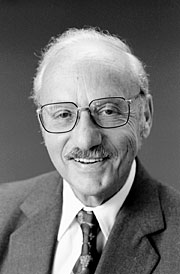
\includegraphics[width=\textwidth]{images/dantzig.jpg}
    \end{column}
\end{columns}
\end{frame}

%% --------------------------------------------------------

\begin{frame}{Algoritmo Simplex}

Durante seu desenvolvimento, Dantzig viu a oportunidade de minimizar/maximizar uma função objetivo
\begin{itemize}
    \item Assim, ao invés de simplesmente resolver sistemas lineares, foi possível otimizar a solução destes sistemas
\end{itemize}

\vspace{1cm}

Assim, nascia a programação linear!
\end{frame}

%% --------------------------------------------------------

\begin{frame}{Complexidade do algoritmo Simplex}

\begin{columns}[T]
    \begin{column}{.43\textwidth}
    Problemas de programação linear podem ser resolvidos em tempo polinomial

    \vspace{0.5cm}
    
    Entretanto, o Simplex é um algoritmo exponencial! \href{https://en.wikipedia.org/wiki/Klee\%E2\%80\%93Minty\_cube}{\beamergotobutton{Link}}
    \begin{itemize}
        \item Demonstrado em um caso extremamente particular
        \item Politopo de Klee–Minty 
    \end{itemize}

    \vspace{0.5cm}
    
    No caso médio, ele tem tempo polinomial
    
\end{column}
    \begin{column}{.56\textwidth}
    \vspace{1cm}
    \centering 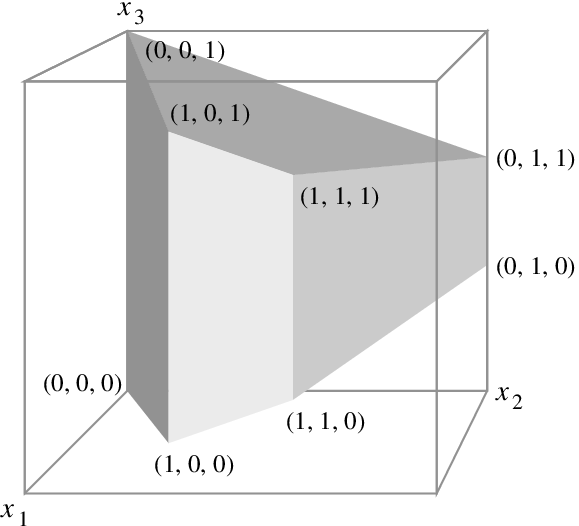
\includegraphics[width=\textwidth]{images/km_cube.png}
    \end{column}
\end{columns}


\end{frame}

%% --------------------------------------------------------

\begin{frame}{Visualização do algoritmo Simplex}

\vspace{1cm}

\centering 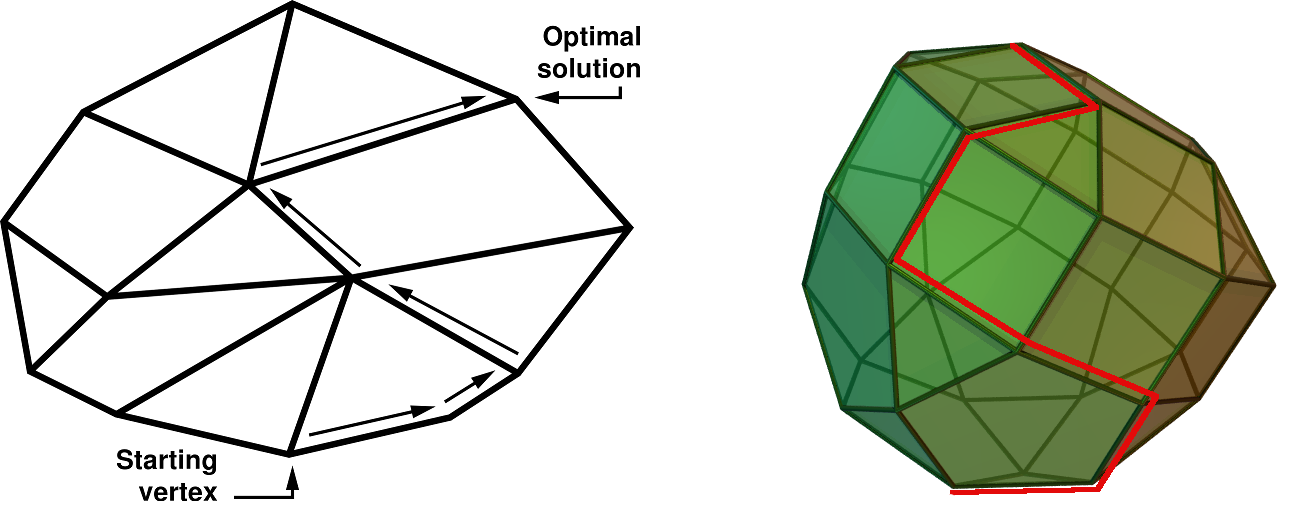
\includegraphics[width=\textwidth]{images/simplex_path.png}

\end{frame}

%% --------------------------------------------------------

\begin{frame}{Tableau Simplex}

  $$\begin{matrix}
        \min & c^Tx \\ 
             & Ax + y & = B \\
             & x & \geqslant 0 \\
             & y & \geqslant 0
        \end{matrix}    
$$

onde 
\begin{columns}[T]
    \begin{column}{.49\textwidth}
    \vspace{0.7cm}
    $A = \begin{bmatrix}
a_{11} & a_{12} & \dots & a_{1n}\\ 
a_{21} & a_{22} & \dots & a_{2n}\\ 
\vdots & \vdots & \ddots & \vdots \\ 
a_{m1} & a_{m2} & \dots & a_{mn}
\end{bmatrix}$ \\
\vspace{0.5cm}
$c = \{c_1, c_2, \ldots, c_n\}$ \\
\end{column}
    \begin{column}{.49\textwidth}
    \vspace{0.25cm}
    $x^T = \{x_1, x_2, \ldots, x_n\}$ \\
    \vspace{0.45cm}
    $B^T = \{b_1, b_2, \ldots, b_m\}$ \\
    \vspace{0.45cm}
    $y = \begin{bmatrix}
        y_{1} & 0 & \dots & 0\\ 
        0 & y_{2} & \dots & 0\\ 
        \vdots & \vdots & \ddots & \vdots \\ 
        0 & 0 & \dots & y_{m}
    \end{bmatrix}$
\end{column}
\end{columns}

\end{frame}

%% --------------------------------------------------------

\begin{frame}{Tableau Simplex}

Modelo linear
$$\begin{matrix}
        \min & c^Tx \\ 
             & Ax + y & = B \\
             & x & \geqslant 0 \\
             & y & \geqslant 0
        \end{matrix}    
$$

\vspace{1cm}

Tableau Simplex

$$\begin{bmatrix}
1 & -c^T & 0_{|m|} & 0\\ 
0 & A & y & B 
\end{bmatrix}$$

\end{frame}

%% --------------------------------------------------------

\begin{frame}{Tableau Simplex}

Modelo linear
$$\begin{matrix}
        \min & -2x - 3y - 4z \\ 
             & 3x + 2y + z & \leq 10 \\
             & 2x + 3z & \leq 15 \\
             & x & \geqslant 0 \\
             & y & \geqslant 0 \\
             & z & \geqslant 0 
        \end{matrix}    
$$

\vspace{1cm}
Tableau \\ 
\centering 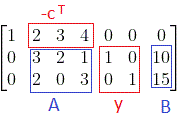
\includegraphics[width=0.3\textwidth]{images/tableau.png}

\end{frame}






\end{document}